\documentclass[12pt]{article}
\usepackage[usenames,dvipsnames]{color}
\usepackage{listings}
\usepackage{graphicx}
\usepackage{fancyhdr}
\usepackage{framed}
\usepackage[T1]{fontenc}
\usepackage[toc,page]{appendix}
\usepackage[utf8]{inputenc}
\usepackage[brazil]{babel}
\usepackage{fancyvrb}
\usepackage[hmargin=2cm,vmargin=2cm]{geometry}
\usepackage{lastpage}
\usepackage{pdfpages}
\usepackage{makeidx}
\usepackage{hyperref}
\pagestyle{fancy}
\usepackage{enumitem}
% cabecalho e rodapé
\setlength{\headheight}{120pt}
\setlength{\textheight}{550pt}
\renewcommand{\headrulewidth}{0pt}
\lhead{
\includegraphics[scale=0.03]{brasao.png}}
%\chead{\includegraphics[scale=0.5]{logo-brasil-sem-pobreza2.png}}
\rhead{
\includegraphics[scale=0.5]{logo-pnud.png}}
\cfoot{\textbf{\ProjectCode\ - Inovando a democracia participativa}}
\rfoot{\thepage}

\hyphenation{par-ti-ci-pa-ção}
\bibliographystyle{ieeetr}

% definições sobre o autor e o produto
\newcommand{\MyName}{Renato Fabbri}
\newcommand{\MySurnameForename}{Fabbri, Renato}
\newcommand{\SupervisorName}{Ricardo Poppi}
\newcommand{\MyEmail}{renato.fabbri@gmail.com}
\newcommand{\ContractNumber}{2013/000566}
\newcommand{\ContractYear}{2014}
\newcommand{\ProjectCode}{Projeto BRA/12/018}
\newcommand{\NomeSecretaria}{Secretaria-Geral da Presidência da República}
%Q\newcommand{\SiglaSecretaria}{SG/PR}
\newcommand{\SiglaSecretaria}{Secretaria: SNAS }
\newcommand{\ProductNumber}{04}
\newcommand{\ProductTitle}{Proposta de adaptações e incrementos para a interface do portal federal de participação social e suas ferramentas}
\newcommand{\ProductSubtitle}{com elementos visuais e de usabilidade para mecanismos de priorização de conteúdos e autorregulação}
\newcommand{\ProductDescription}{"Proposta de adaptações e incrementos para a interface do portal federal de participação sociais e suas ferramentas, com elementos visuais e de usabilidade para mecanismos de priorização de conteúdos e auto-regulação"}

\newcommand{\ProductValue}{R\$ 21,600 (vinte e um mil e seiscentos reais)}
\newcommand{\ObjetoContratacao}{
Aporte de conhecimentos e tecnologias para especificação de vocabulário e ferramentas assistidas que utilizam processamento de linguagem natural e análise de redes complexas para o conteúdo do portal da participação social.
}
\newcommand{\DataEntrega}{10 de Setembro de 2014}
\newcommand{\PalavrasChave}{reconhecimento de padrões, redes complexas, processamento de linguagem natural, participação social}

% lista de abreviações
\makeindex

\begin{document}


\newgeometry{hmargin=3cm,vmargin=1.5cm}
\begin{center}
\thispagestyle{empty}
{\color{MidnightBlue}


\includegraphics[scale=0.9]{logo-pnud.png}

\vspace{4cm}

{\bf \large \ProjectCode\ - Desenvolvimento de Metodologias
de Articulação e Gestão de Políticas Públicas para Promoção da Democracia
Participativa}

\vspace{1.5cm}

{\bf \large Produto \ProductNumber\ -\ \ProductTitle}

\vspace{1.5cm}

\ProductSubtitle

\vspace{4cm}

\MyName

\vspace{1cm}

}


\includegraphics[scale=0.04]{brasao.png} \\
{\bf \small \NomeSecretaria}

\end{center}
\restoregeometry
\newpage

\newgeometry{hmargin=3cm,vmargin=1.5cm}
\addtolength{\topmargin}{2.5cm}
\thispagestyle{empty}
{\color{MidnightBlue}

{\bf \LARGE Produto \ProductNumber\ -\ \ProductTitle}

\hrulefill

\vspace{1cm}

\begin{center}

{\bf \large Contrato n. \ContractNumber}

\vspace{1.5cm}

{\bf \large Objeto da contratação: \ObjetoContratacao}

\end{center}

\vspace{3.2cm}

Valor do produto: \ProductValue

\vspace{1.2cm}

Data de entrega: \DataEntrega

\vspace{1.2cm}

Nome do consultor: \MyName

\vspace{1.2cm}

Nome da supervisora: \SupervisorName

}

\vspace{2cm}

\begin{center}

\includegraphics[scale=0.04]{brasao.png} \\
{\bf \small \NomeSecretaria}
\end{center}

\restoregeometry
\newpage

\newgeometry{hmargin=3cm,vmargin=1.5cm}
\addtolength{\topmargin}{5cm}
\thispagestyle{empty}

\begin{framed}

{\raggedright \MySurnameForename} \\

\ProductTitle: \ProductSubtitle\ / \ContractYear. \\

Total de folhas: \pageref{LastPage} \\

\vspace{1cm}

Supervisor(a): \SupervisorName \\

\SiglaSecretaria \\

\NomeSecretaria \\

Palavras-chave: \PalavrasChave. \\

\end{framed}

\vspace{3cm}

{\raggedright 
\includegraphics{licenca-cc-by-nc.png} \ Esta obra é licenciada sob
uma licença Creative Commons - Atribuição-NãoComercial. 4.0 Internacional.}

\restoregeometry
\newpage

\tableofcontents
\newpage


\begin{abstract}
Este documento descreve rotinas de priorização de conteúdo e de autorregulação para o portal federal de participação social. Como parte da exposição e do Produto, foi implementado um sistema de recomendação de participantes para outros participantes e linha editorial do participa.br. Este sistema está online e visa atender a requisitos como os do ActionItem 3234 do Noosfero, que prevê recomendação de participantes, comunidades e empreendimentos. Como generalização da proposta, é delineada  recomendação de recursos como trilhas, artigos, comentários e palavras. O consultor e equipe do participa.br entendem que a disponibilização destes recursos em formato aberto - e com documentações reativas para fácil geração de derivados, críticas e propostas - é instrumental para a democracia participativa e online, promovendo empoderamento e transparência.\\

{\bf Palavras-chave:} \PalavrasChave.
\end{abstract}
\newpage

\section{Introdução}
\subsection{Contexto e importância da consultoria}
Em confluência com o portal federal de participação social (Participa.br) e o Plano Nacinal de Participação Social (PNPS), esta consultoria é um aporte de conhecimentos e tecnologias de web semântica, redes complexas e processamento de linguagem natural. O presente produto apresenta ``formas de priorização de conteúdo e de autorregulação'' na forma de um sistema de recomendação de recursos para participantes e linha editorial. No começo da seção~\ref{sec:dev} está explicitada a motivação para a implementação e a relação com o cumprimento dos termos deste Produto~\cite{termoReferencia}.

\subsection{Contexto e importância do Produto}
\subsubsection{Objetivos}
Este produto tem por objetivo principal a disponibilização de um sistema de recomendação de recursos do participa.br para usuários, tanto via critérios personalizados quanto considerando comunidades e linha editorial. Através deste sistema de recomendação, ficam facilitados, até mesmo prontamente disponíveis, diversos processos de autorregulação, de geração de resumos, de geração de relatórios e de análises informativas. Objetivos secundários são:
\begin{itemize}
    \item Disponibilização de uma API HTTP, para uso no participa.br, conforme requisitado pela equipe do Participa.br em diversos itens dos produtos~\cite{prodExtra}.
    \item A exposição destes algoritmos de recomendação aos visitantes web via uso de browsers comuns, para edição e execução dos trechos de código utilizados pela plataforma federal de participação social. Este objetivo foi satisfeito usando o IPython Notebook levantado para este trabalho~\cite{iNotebook}.
    \item Aproveitamento do endpoint SparQL com os dados do participa.br, fortalecendo as tecnologias de dados linkados e web 3.0~\cite{endpoint}.
    \item Em reunião com a consultora Daniela Feitosa, foi delineada a pertinência de um sistema de recomendação de perfis para um ActionIntem em andamento para o participa.br~\cite{actionItem}. Este produto visa suprir esta necessidade através da API disponibilizada para recomendações.
    \item A entrega das tecnologias livres com simplicidade e boa documentação, favorecendo o aproveitamento deste trabalho para melhoras, geração de derivados e novas e independentes tecnologias. Isso pode ser observado no repositório git público deste produto~\cite{repoProd4}.
    \item Compatibilizar ao máximo a entrega deste produto às demandas da equipe do participa.br~\cite{prodExtra}.
    \item Realizar de forma precisa e pertinente a especificação deste quarto produto no Termo de Referência~\cite{termoReferencia}.
\end{itemize}

\subsubsection{Resultados esperados}
De imediato e mais central, o resultado do produto é iniciar um processo aberto de desenvolvimento e apropriação de análises e mecanismos de autorregulação para o portal federal de participação social.

Como resultados diretos deste Produto, constam:
\begin{itemize}
    \item a habilitação para uso da API HTTP para recomendação de recursos do participa.br. Veja Apêndice~\ref{sec:api2},~\ref{sec:infra} e~\ref{sec:inst}.
    \item A interface para apreensão e inovação dos algoritmos, não somente exemplificada ou projetada, mas operante e disponível. Veja Apêndice~\ref{sec:algs}.
    \item Um plano de implementação para o participa.br, que utiliza a API de recomendação para priorização de conteúdo e autorregulação. Veja Apêndice~\ref{sec:acr}.
    \item Transparência absoluta no trabalho, com toda a documentação e código computacional online em um repositório git que contem o histórico de implementação~\cite{repoProd4}.
    \item Algoritmos implementados em código de simples leitura, para facilitar a implementação em outras linguagens como Ruby ou Javascript, quando houverem recursos mais maduros para estas linguagens ou por necessidade. No momento, Python possui mais e mais maduros recursos tanto para redes complexas quanto para processamento de linguagem natural.
    \item Habilitação de implementações em andamento, como o plugin de recomendação de perfis~\cite{actionItem}, para recomendar amigos para participantes. 
\end{itemize}
\subsubsection{Caráter inovador}
Centralmente, este trabalho é inovador na aplicação de recursos de análise de redes sociais para empoderamento da sociedade civil, entregando as tecnologias e priorizando a reutilização. Este recurso é de vital interesse para a democracia participativa no contexto atual, com as revoluções da internet e das redes sociais. Permite, em última instância, que haja uma inteligência para aproveitamento das estruturas sociais, e que esta inteligência seja pública, transparente, minimizando vetores vigilantistas ou turvos.

Há a inovação na arquitetura em software, apresentando traços de web 3.0 como os dados linkados como base de conhecimento e os múltiplos recursos online acessados no funcionamento usual (ao menos Endpoint SparQL para acesso aos dados, API HTTP Flask para tratar os dados e gerar estatísticas e estruturas de interesse, Participa.br para interface e contexto pertinente).

Há inovação na difusão científica. Além dos métodos e tecnologias disponibilizadas, por exemplo, os termos Web Semântica, Processamento de Linguagem Natural e Redes Complexas são empregados em textos científicos e consistem em áreas que recebem pesquisas, revistas e até carreiras científicas inteiras. Neste Produto, este conteúdo está apresentado em português e se presta a facilitar contribuições de outras partes interessadas.

Os métodos de recomendação em si não foram confrontados exaustivamente com a literatura, mas possivelmente possuem também inovações nos procedimentos. Certamente há inovação no contexto de implementação, tanto de relevância social (portal federal de participação social) quanto de aparato tecnológico (web 3.0, métodos da física e de mineração de dados).

\subsubsection{Aparato em software e hardware}\label{subsec:hs}


O sistema de recomendação precisa ser mantido online, e isso implica na manutenção de uma estrutura em hardware e software que extrapola o objeto deste produto. As especificações desta arquitetura de software e hardware estão em um documento escrito pelo consultor a pedido da PR para a SNAS e DITEC~\cite{smDITEC}. Para fins de pesquisa e de entrega deste produto, o esquema da Figura~\ref{fig:sr} é realizado em máquinas de pesquisa da USP, concedidas para a pesquisa de doutorado do consultor. Tal configuração é razoável pois a pesquisa conflui e é potencializada por esta consultoria, mas está prevista uma infraestrutura própria da PR para estes serviços. Além disso, os usos atuais ainda são moderados, sem causar sobrecarga ao serviços de computação em nuvem da USP.

\begin{figure}[h!]
  \centering
      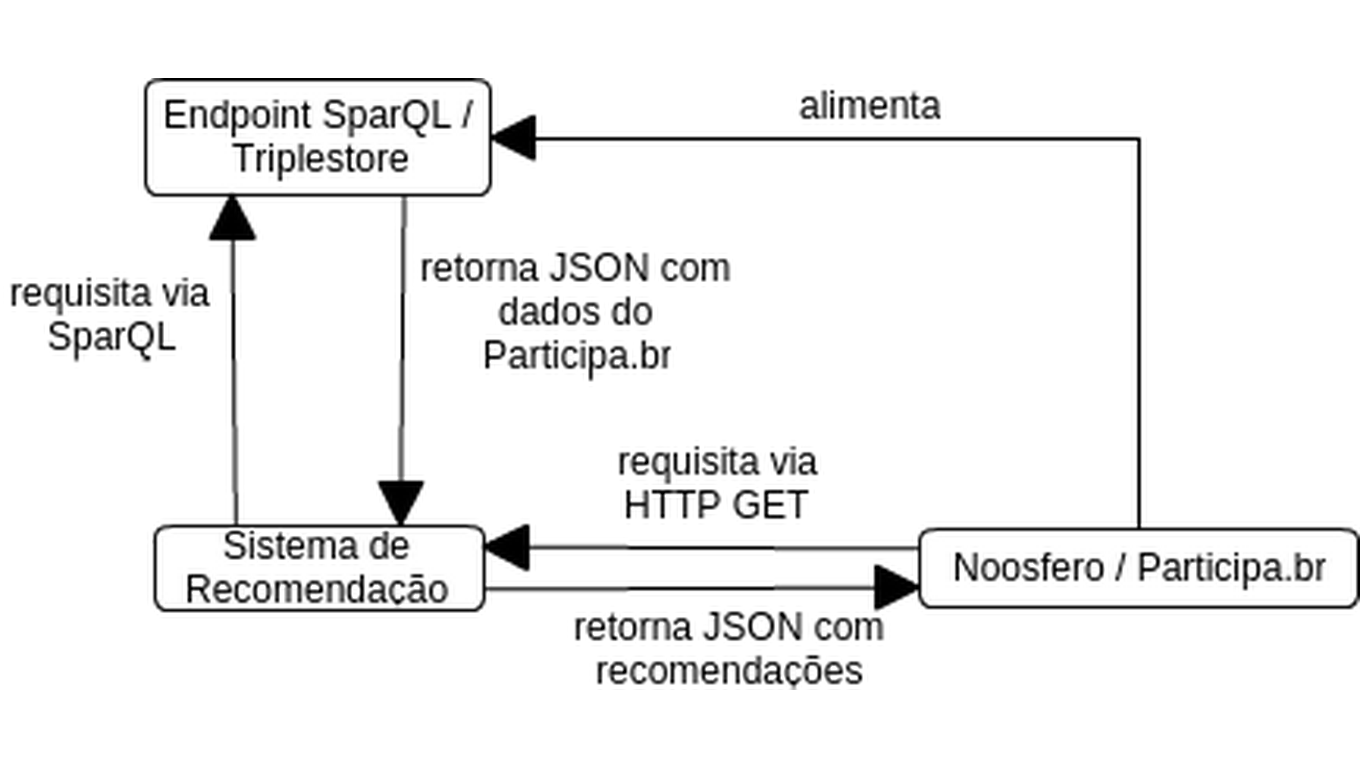
\includegraphics[width=0.8\textwidth]{sr}
  \caption{O sistema de recomendação e relações principais: com o frontend Participa.br e com a base de dados enriquecidos semanticamente.}\label{fig:sr}
\end{figure}

\section{Desenvolvimento}\label{sec:dev}
O produto é descrito no Termo de Referência desta consultoria assim: ``Documento com proposta de adaptações e incrementos para a interface do portal e suas ferramentas que inclua elementos visuais e de usabilidade para mecanismos de priorização de conteúdos e auto-regulação com base nos metadados gerados nativamente pela plataforma do portal e nas análises de PLN e RC produzidas pelas ferramentas assistidas''.

Dada a dimensão do participa.br, tanto da estrutura em software e das práticas participativas, quanto de mobilização humana, as propostas de adaptações para o portal são muitas e estão em diversos produtos deste e de outros consultores. Uma forma especialmente pertinente de realizar este produto, confluente com o Termo de Referência desta consultoria, com o trabalho dos gestores e comunidade e com os produtos deste e de outros consultores~\cite{prodExtra}, é a entrega de um sistema de recomendação de recursos para o participa.br.

Conforme discutido em reunião com gestores e comunidade do participa.br~\cite{padProd4}, em termos de \emph{priorização de conteúdo}, quase todos os casos de interesse para o atual participa.br podem ser considerados rotinas de recomendação. Além disso, dadas as práticas atuais de redes sociais, os mecanismos de autorregulação do participa.br são e serão baseados na adição de conteúdo por espontaneidade dos participantes. Esta dinâmica de adição espontânea de conteúdo pelos participantes conflui com sistemas de recomendação de recursos, pois estes podem catalizar sem coerção os processos participativos.

Desta forma, foi idealizada a entrega de um sistema de recomendação de recursos do participa.br para seus usuários, comunidades e linha editorial. As subseções a seguir apontam etapas na construção do sistema de recomendação. Os Apêndices~\ref{sec:api} e~\ref{sec:algs} concentram aspectos de operação do sistema. Os Apêndices~\ref{sec:infra} e~\ref{sec:inst} são voltados para os componentes e a instalação da versão operante deste sistema de recomendação de recursos. A seção~\ref{sec:uso} e o Apêndice~\ref{sec:acr} apreendem previsões e propostas de integração com o participa.br.

\subsection{Etapas de desenvolvimento anteriores a este produto}
\subsubsection{Sistematização ontológica da participação online}
Através de estudos e reuniões presenciais e online, a Ontologia de Participação Social (OPS) foi revisada~\cite{OPS} e a Ontologia do Participa.br (OPA) foi feita~\cite{OPA}.
\subsubsection{Triplificação dos dados do participa.br}
Feito um script para triplificar os dados do Participa.br, ou seja, para o enriquecimento semântico e escrita em RDF dos dados em Postgresql da instância Noosfero do Participa.br~\cite{triplifica}.
\subsubsection{Levantamento do endpoint SparQL}\label{sec:sfoo}
Para uso dos dados triplificados, pode-se recorrer a diversos métodos de leitura e disponibilização. Um método-chave é a disponibilização dos dados rdf (\emph{triple store}) em um \emph{endpoint sparql}. Para os fins de testes, pesquisa e usos leves, está disponibilizado um endpoint SparQL em servidores da USP~\cite{endpoint}.
\subsubsection{Análises iniciais, modelos}
Análises dos dados do participa.br foram abertas no IPython Notebook, com ênfase no texto produzido e nas redes formadas~\cite{repoProd3}.
\subsection{Etapas de desenvolvimento deste produto}
\subsubsection{Reuniões com equipe do participa.br}
Especial agradecimentos ao Ricardo Poppi, Ronald Costa, Enaile Ladanza, Joênio Costa, Daniela Feitosa e Fernando Cruz.
\subsubsection{Estudos de aprofundamento e amadurecimento}
Em especial, foram lidos todos os produtos entregues pelos consultores, (re)visitados cursos no coursera e literatura científica~\cite{prodExtra}.
\subsubsection{Escrita deste documento}
Através da escrita deste documento, várias informações foram organizadas e sistematizadas, facilitando compreensão do contexto para especificação da API de recomendação e entrega do produto.
\subsubsection{Especificação da API de recomendação}\label{sec:api3}
Basicamente, é convencionado um padrão na montagem das URLs para recomendar recursos de tipos especificados, para destinatários e por métodos também especificados. O Apêndice~\ref{sec:api} é dedicado a expor a convenção inicial entre URLs formadas e as recomendações que retornam.
\subsubsection{Implementação do serviço para aquisição dos dados, processamento e entrega em JSON}
Para a API da etapa acima, foi necessário desenvolver um servidor HTTP simples (em Flask). Veja pasta flask/ de~\cite{repoProd4}. 
\subsubsection{Disponibilização das rotinas no IPython Notebook}\label{sec:inb5}
Para expor os critérios de recomendação, disponibilizar análises e facilitar novas versões para as recomendações, as rotinas estão em um IPython Notebook. Veja o Apêndice~\ref{sec:algs} para uma exposição e detalhamento destas rotinas.
\subsubsection{Proposta de implementações no portal federal de participação social}
Com base no sistema de recomendações, nas demandas levantadas em reuniões e nos produtos já feitos por este e outros consultores, foi sistematizado um conjunto de propostas de acréscimos para o portal federal, detalhado no Apêndice~\ref{sec:acr}.
\subsection{Justificativa do método}
São usados diversos métodos neste produto. As justificativas se concentram nas tecnologias de web 3.0 (dados linkados e computação em nuvem), nas técnicas mais fundamentais/básicas/simples e nas demandas da equipe do participa.br, observadas através de reuniões e documentações produzidas recentemente pela equipe~\cite{prodExtra}.
\subsection{Justificativa das fontes}
A equipe do participa.br é uma equipe estratégica da Presidência da República voltada para participação social. As fontes externas utilizadas, como artigos, livros e videos, são garimpadas como atual pesquisa acadêmica principal do consultor.
\subsection{Confronto entre os resultados esperados e os alcançados}
No Termo de Referência desta consultoria, este produto é descrito como ``Documento com proposta de adaptações e incrementos para a interface do portal''. Este produto entrega estas propostas a serem implementadas no portal federal de participação social. Além disso, para facilitar estas implementações e fazer a conexão com os desenvolvimentos ontológicos e de dados linkados, foi implementado e disponibilizado um sistema de recomendação de recursos para o participa.br. Um outro resultado para além do esperado, é a consideração cuidadosa da comunidade de democracia participativa, com a disponibilização das rotinas de recomendação no IPython Notebook~\cite{iNotebook} e uma visita aos produtos dos outros consultores~\cite{prodExtra}.

\section{Usos dos resultados}\label{sec:uso}
Há usos previstos do sistema de recomendação, pois são demandas da equipe que motivaram o seu desenvolvimento. Em especial, há o uso previsto no plugin de recomendação de perfis (ActionItem~\cite{actionItem}).

Há usos próprios dos participantes, como consultas aos recursos recomendados para si e para outros, e usos para a linha editorial do portal. Estes usos podem ser feitos no próprio servidor que disponibiliza o serviço de recomendação. Podem ser adaptados para a interface do participa.br, com plugins ou temas apropriados. Algumas sugestões de implementações estão no Apêndice~\ref{sec:acr}.

Outro uso previsto, e que idealmente contará com incentivos da comunidade, é a evolução destes métodos de recomendação de perfis para melhor atender aos usos do portal e das comunidades. O consultor sugere que as comunidades sejam convidadas a apresentar uma ou mais pessoas com conhecimentos ou diposição para algoritmos e sistematizações. Esta pessoa poderia passar, por exemplo, por uma reunião para apreensão dos métodos de recomendação e análise, com vistas a proposição de melhoras e ampliação das funcionalidades.

As rotinas de recomendação estarão disponíveis online, e editáveis e executáveis no browser via IPython Notebook, o que deve facilitar dinâmicas de compartilhamento e amadurecumento destes processos. Este uso dos resultados deste produto é ainda mais central do que a API em si ou o uso dela dentro do participa.br. Mesmo assim, dada a complexidade das técnicas usadas, das tecnologias envolvidas e dos propósitos, o uso da API dentro do participa.br trará menos desafios que a apreensão, aproveitamento e melhora destes métodos pela comunidade de democracia participativa. Por isso, fica reforçada a pertinência da atenção da comunidade. 

Um uso previso é a potencialização de uma biblioteca digital, incluindo buscas e recomendações no participa.br. Também sobre biblioteca digital, mas agora na alimentação dela, análises dos dados do participa.br podem ser feitas diariamente e constar como documentos da biblioteca digital. Outras análises especiais podem entrar como itens na biblioteca digital, facilitadas com as rotinas já disponibilizadas, e facilitando posteriores.

\section{Conclusão}
\subsection{Comentários, sugestões, recomendações}\label{subsec:com}
O consultor recomenda que haja amadurecimentos em encontros, tanto para melhora deste legado do participa.br, quanto para apreensão dos métodos pelas comunidades interessadas. 

As estruturas básicas para as análises e recomendações, que são as redes (de amizade e de interação) e os histogramas de palavras, podem ser convenientemente incluidos na triplificação dos dados, de forma que as recomendações e análises fiquem mais leves. Por hora, para viabilizar o uso, o sistema de recomendações refaz estas estruturas caso seja visitado o caminho \url{recomenda/atualiza}. Estas estruturas são:
\begin{itemize}
    \item Rede de amizades.
    \item Rede de interação.
    \item Histograma de radicais das palavras de todos os textos (artigos e comentários) do participa.br.
    \item Seleção dos 400 radicais mais ocorrentes para caracterizar o domínio.
    \item Histograma de radicais de cada usuário e contagem das ocorrências das palavras selecionadas para caracterizar o domínio.
\end{itemize}

Os métodos de recomendação implementados utilizam separadamente critérios linguísticos ou de interação/relacionamento. Os casos e resultados
já são interessantes e até complexos para uma primeira versão. Há implementações delineadas 
que utilizam ambos recursos linguísticos e de relacionamento (topológicos). Por hora, ambas as características podem ser
utilizadas operando as pontuações das recomendações com base no texto com pontuações das recomendações com base em interação/relacionamento.

\subsection{Impacto do Produto para a elaboração, gestão e/ou avaliação de políticas públicas de participação social}
Este trabalho torna disponível uma porção de avaliações automáticas dos processos participativos que ocorreram ou ocorrerem no participa.br. Estas mesmas avaliações podem ser usadas continuamente, facilitando a gestão. A elaboração pode se beneficiar da análise das experiências passadas, facilitada pelos métodos aqui presentes.

Outro impacto pra a elaboração e gestão é basear o método de participação na utilização de métodos de recomendação de recursos. Por exemplo: pode-se recomendar que participantes com características X faça provocações. Estas provocações são enviadas para outros participantes como recomendações. Ainda a outros participantes pode ser recomendada a sistematização destes resultados. Um exemplo mais próximo da democracia participativa atual é uma etapa em que os participantes escrevem para recomendados participantes para fazer contato e iniciar discussões.

Para a gestão, pode ficar facilitado o fomento e a qualificação da participação. Por exemplo, o plugin de recomendação de amigos~\cite{actionItem} deixa o portal mais interessante para o participante, pois apreende melhor seus relacionamentos e expõe os critérios de busca como instrumentos para sua participação. 

\subsection{Como o Produto deverá impactar o público-alvo das políticas públicas a que se refere}
As comunidades afeitas à participação social poderão aproveitar estas análises para melhor assimilação dos processos participativos, para relatórios, para gerar novos métodos de recomendação que melhor atendam aos interesses específicos das comunidades ou aos interesses da democracia participativa.

Um impacto imediato é a transparência reforçada dos processos participativos, pois não somente os dados, mas as análises e as recomendações dos recursos do participa.br estão online e publicamente disponíveis para geração de derivados.

Outro impacto imediato é a valorização da participação. Sempre que um participante, por exemplo, fizer uma amizade ou comentar uma postagem ou outro comentário, ele estará constando nas redes envolvidas, modificará as análises atuais, e poderá ver seu nome e de outros em relações diversas.

\section{Agradecimentos}
O consultor Renato Fabbri agradece ao Joenio Costa pelo template em \LaTeX para os produtos. Agradece à Daniela Feitosa pela reunião para demanda de recomendação de perfis. Agradece aos supervisores do trabalho realizado em torno do participa.br: Ricardo Poppi e Ronald Costa. Agradece ao labMacambira.sf.net e todas as comunidades de software e cultura livre que compõe esta contribuição.
\newpage
\bibliography{bibliografia}
\newpage
%\listoffigures
\section*{Abreviações e jargão}
\begin{itemize}[label={}]
    \item {\bf RC:              } Redes Complexas
    \item {\bf PLN:             } Processamento de Linguagem Natural
    \item {\bf OPS:             } Ontologia de participação Social
    \item {\bf OPA:             } Ontologia do Participa.br
    \item {\bf MMISSA:          } Monitoramento Massivo e Interativo da Sociedade pela Sociedade para Aproveitamento
    \item {\bf AARS:            } A Análise de Redes Sociais
    \item {\bf MyNSA:           } Monitoring yields Natural Streaming and Analysis
    \item {\bf PNPS:            } Plano Nacional de Participação Social
    \item {\bf RDF:             } Resource Description Framework
    \item {\bf HTTP:            } Hypertext Transfer Protocol
    \item {\bf SPARQL:          } Simple Protocol and RDF Query Language
    \item {\bf endpoint SPARQL: } ponto de acesso, geralmente HTTP, a dados em RDF via buscas em SPARQL.
    \item {\bf Participa.br:    } Portal federal de participação social.
    \item {\bf IPython Notebook:} instância online para rodar scritps Python
    \item {\bf Meteor:          } arcabouço para páginas reativas e com funcionamento distribuído.
    \item {\bf D3js:            } biblioteca de visualização de dados.
\end{itemize}

\newpage
\printindex
\newpage
%\input{listadeanexos.tex}
\appendix
\section{Especificação da API de recomendação de recursos do participa.br}\label{sec:api}
As rotinas no Apêndice~\ref{sec:algs} podem ser adaptadas para os mais diversos fins. No sistema de recomendação disponibilizado há quatro campos principais e dois auxiliares:
\begin{itemize}
    \item Recurso: o recurso a ser recomendado: participantes, comunidades, trilhas, artigos ou comentários.
    \item Destinatário: para quem está sendo feita a recomendação: participante, comunidade ou linha editorial. Campo auxiliar ``idd'' para id do destinatário (comunidade ou participante).
    \item Método: método para a recomendação: ``topologico'', ``textual'' ou ``hibrido''. Campo auxiliar de polaridade similar, dissimilar ou mista.
\end{itemize} 
A url usada para consulta HTTP incorpora os parâmetros da forma usual:
\url{http://<urlDoServidor>/recomenda?recurso=participante&destinatario=linha_editorial&metodo=topologico&polaridade=mis&ordenacao=embaralhada}
\subsection{Instância online e especificações}
\subsection{Aspectos operantes}
No momento de entrega deste produto, estão implementadas recomendações para os casos apontados na Tabela~\ref{tab:srCampos}

\begin{table}
\begin{center}
\begin{tabular}{|l|l|p{10cm}|}\hline
\textbf{campo} & \textbf{opções} & \textbf{comentários} \\\hline\hline
\texttt{recurso}       & \texttt{participante} & recomenda participante que são potenciais amigos ou apropriadas para interação \\\hline
\texttt{destinatario}  & \texttt{participante} & o recurso é recomendado para o participante                  \\
                       & \texttt{linha\_editorial} & o recurso é recomendado para a linha editorial do site ou visitante sem registro no participa.br              \\\hline
\texttt{idd}           & \texttt{<id do destinatário>} & {\raggedright id do destinatário caso o destinatário seja um participante. Este id é conforme o campo ``identifier'' da tabela ``profiles'' do Noosfero/Participa.br}           \\\hline
\texttt{metodo}        & \texttt{topologico}  & usar redes de amizades ou interação para fazer as recomendações                   \\
                       & \texttt{textual}    &  usar critérios textuais para fazer as recomendações                   \\
                       & \texttt{hibrido}    &  {\raggedright usar ambos os critérios (topológico e textual) para fazer as recomendações. Por hora retorna ambas as recomendações feitas com base no critérios topológicos e textuais independentemente.} \\\hline
\texttt{polaridade}    & \texttt{simililar}  & retornar recomendações que visam similaridade entre os recursos (potenciais amigos, textos sobre tópicos relacionados, etc)                    \\
                       & \texttt{dissimilar}    & retornar recomendações que visam dissimilaridade entre os recursos (participantes de setores diferentes da rede, vocabulário díspar).                 \\
                       & \texttt{ambas}    & retornar ambas as recomendações similares e dissimilares                      \\\hline
\texttt{ordenacao}     & \texttt{compartimentada} & retorna recomendações agrupadas por critério, na ordem das medições relativas aos critérios, em uma lista de critérios, cada um com um ranqueamento dos recursos e um valor medido. \\
                       & \texttt{embaralhada}    & retorna recomendações embaralhadas, em uma lista de tuplas com três campos: [(recurso, medição, critério),(..),]                \\
                       & \texttt{intercalada}    & {\raggedright retorna recomendações intercaladas, cada uma com um critério diferente, também uma lista de tuplas com três campos:  [(recurso, medição, critério),(..),]       }        \\\hline
\end{tabular}
\caption[Table caption text]{Opções implementadas no atual sistema de recomendação. Por hora, recomenda para participantes e para linha editorial (ou visitantes), via critérios textuais ou topológicos, outros participantes para se articularem, sejam potenciais amigos, parceiros ou oponentes, dependendo dos critérios adotados para a recomendação.}
\label{tab:srCampos}
\end{center}
\end{table}


\begin{table}
\begin{center}
\begin{tabular}{|l|l|p{8cm}|}\hline
\textbf{campo} & \textbf{opções} & \textbf{comentários} \\\hline\hline
\texttt{recurso}       & \texttt{comunidade} & recomenda comunidades de especial interesse para o destinatário \\
                       & \texttt{artigo} & recomenda artigo de especial interesse para o destinatário               \\
                       & \texttt{comentario} & recomenda comentario de especial interesse para o destinatário               \\
                       & \texttt{palavra} & recomenda palavra de especial interesse para o destinatário               \\
                       & \texttt{trilha} & recomenda trilha participativa de especial interesse para o destinatário               \\
                       & \texttt{etapa} & recomenda etapa participativa de especial interesse para o destinatário               \\\hline
\texttt{destinatario}  & \emph{mesmas opções que o campo recursos} & ------    \\\hline
\end{tabular}
\caption[Table caption text]{Opções a serem implementadas no atual sistema de recomendação. O destinatário, de início os participantes e a linha editorial, idealmente é qualquer recurso, a que se destina relacionar as recomendações.
Veja Tabela~\ref{tab:srCampos} para critérios já implementados no momento de entrega deste produto.}
\label{tab:srCampos2}
\end{center}
\end{table}

\subsection{Aspectos planejados}\label{sec:plan}
A Tabela~\ref{tab:srCampos2} relaciona os recursos a serem implementados para o Participa.br.

\subsection{Instância online e exemplos de uso}
Está online uma instância do sistema de recomendação no endereço:
\url{http://200.144.255.210:8081/sr}. Para atualizar estruturas auxiliares (pode demorar mais de 30 minutos de processamento), basta visitar o endereço: \url{http://200.144.255.210:8081/sr/atualiza}. Para realizar consultas, visite \url{http://200.144.255.210:8081/sr/recomenda?<opções via método GET>}.

Exemplos:

A URL \url{http://200.144.255.210:8081/sr/recomenda?recurso=participante&destinatario=linha_editorial&metodo=hibrido&polaridade=ambas&ordenacao=compartimentada} retorna JSON com diversos grupos de participantes recomendados para a linha editorial, por critérios topológicos e textuais.

A URL \url{http://200.144.255.210:8081/sr/recomenda?recurso=participante&destinatario=participante&idd=marcelobranco&metodo=hibrido&polaridade=ambas&ordenacao=compartimentada} retorna JSON com diversos grupos de participantes recomendados para o participante cujo identifier na tabela profiles é marcelobranco.

Embora o sistema deva funcionar normalmente e com os critérios aplicados corretamente, verificações e melhoras devem vir com o uso. Aliás, o consultor está à disposição caso desenvolvedores do Noosfero/Participa.br queiram requisitar dados ou recomendações em formatos que lhes sejam convenientes.

\subsection{Atualização e manutenção}
A URL \url{http://200.144.255.210:8081/sr/atualiza} atualiza as estruturas auxiliares de acordo com os dados disponiveis no endpoint SparQL. O processamento pode levar mais de 30 minutos, de forma que não se deve visitar o link a menos que haja razão para isso. Estas estruturas devem idealmente serem disponibilizadas no endpoint SparQL, junto aos dados do participa.br.
A estrutura pronta pode ser adicionada à \emph{triple store} através do endpoint Jena/Fuseki posteriormente à triplificação dos dados do participa.br. Caso não signifique sobrecarga para a instância do Noosfero/Participa.br, a criação destas estruturas devem ser incluídas no RDF pelo plugin que triplifica os dados do portal, feito por Daniela Feitosa.
\section{Rotinas de acesso e processamento de dados do participa.br para as recomendações}\label{sec:algs}
\subsection{Estruturas auxiliares}
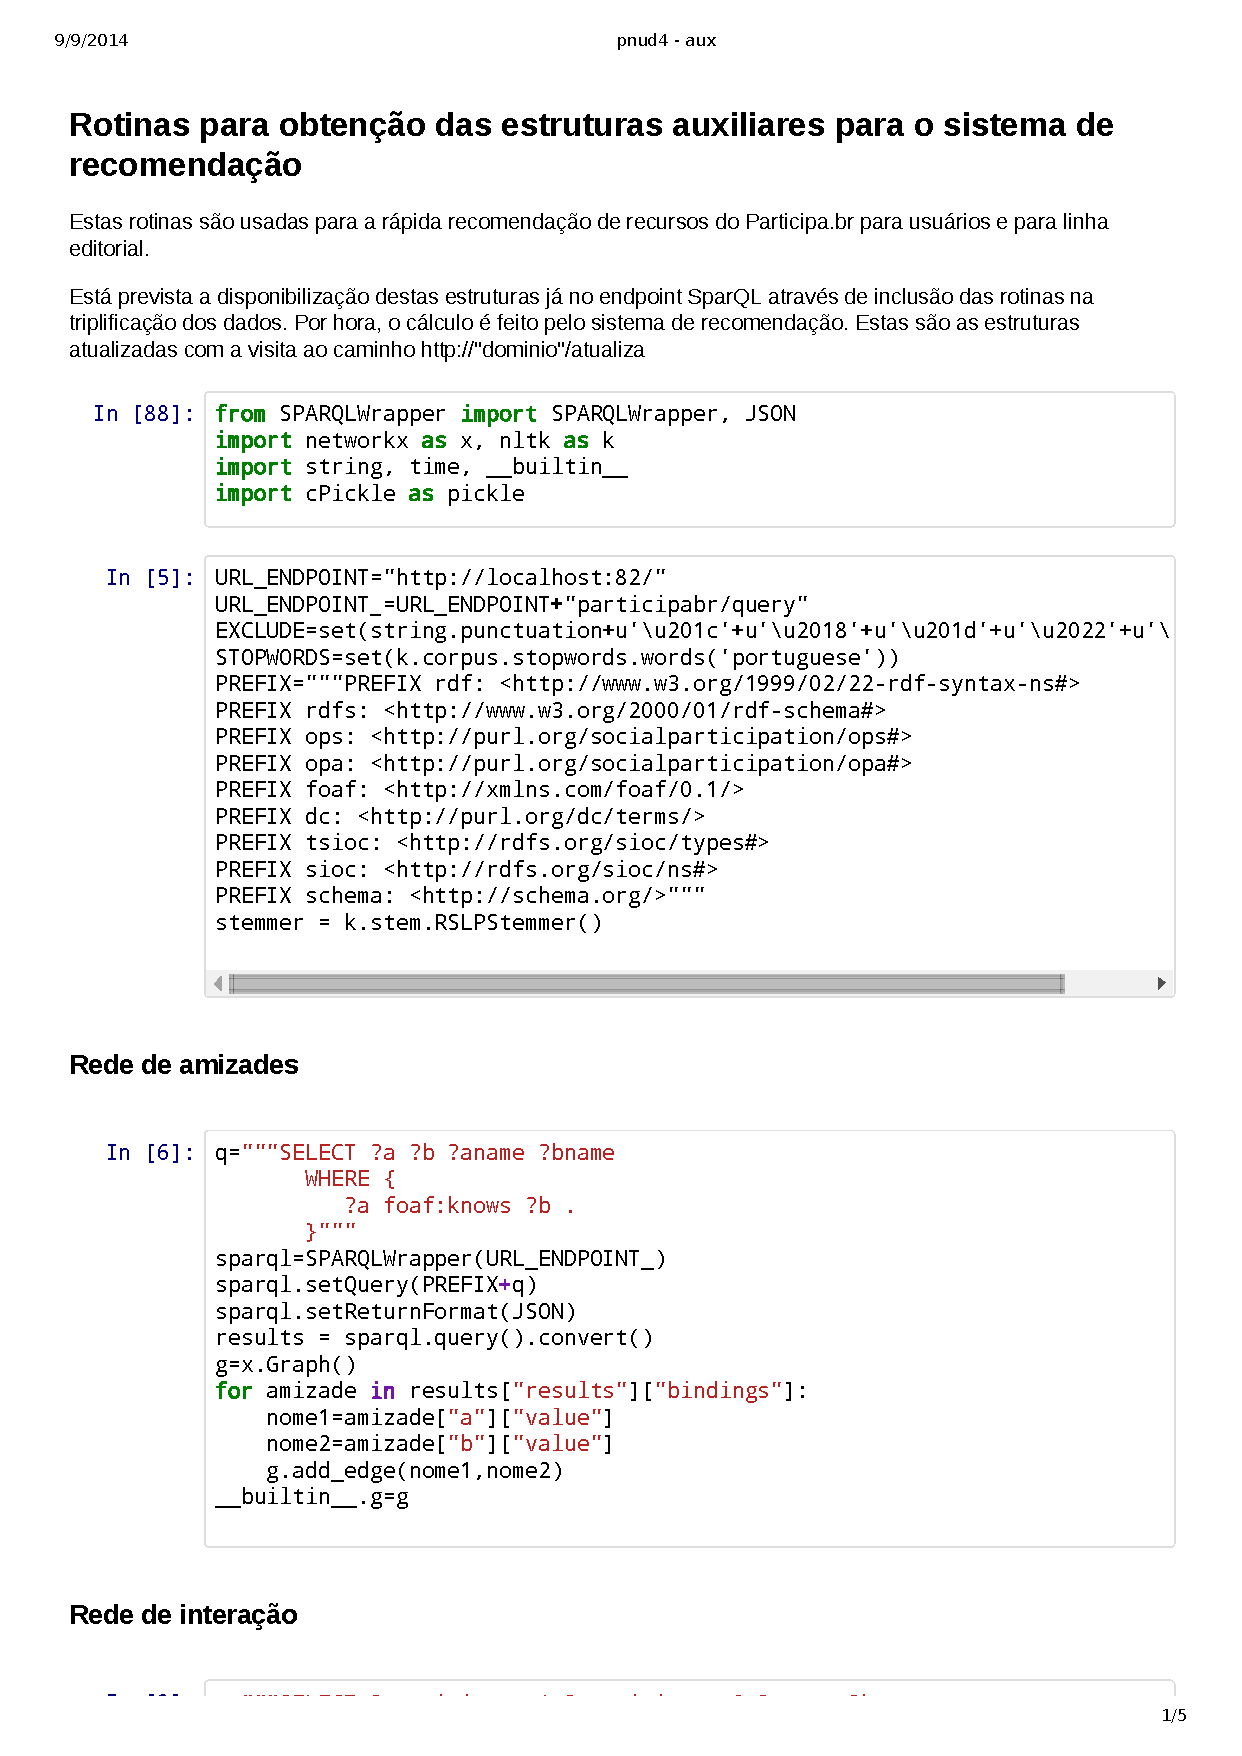
\includepdf[pages=-]{anexos/pnud4aux.pdf}
\subsection{Rotinas para recomendação de recursos}
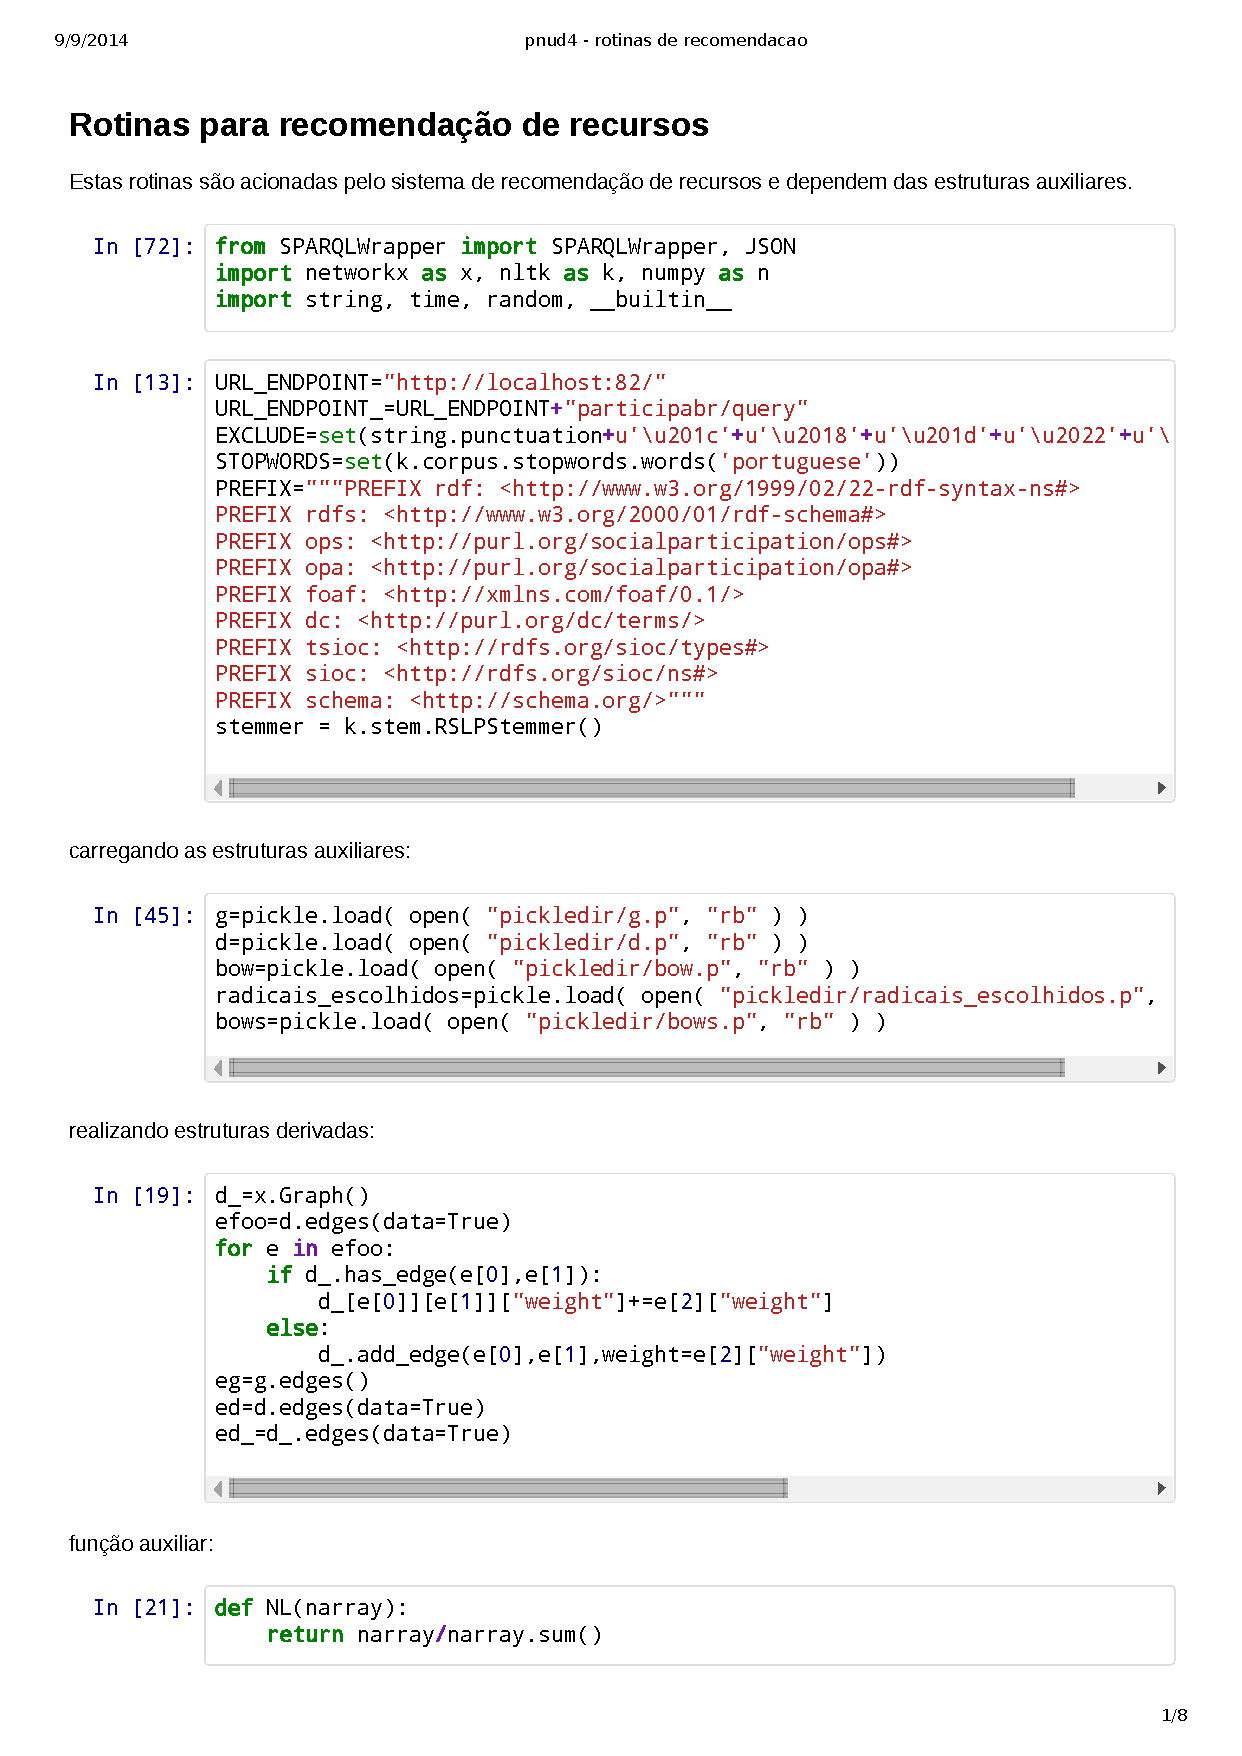
\includepdf[pages=-]{anexos/pnud4rr.pdf}
\section{Parcela dos participantes que produziram texto ou interação}
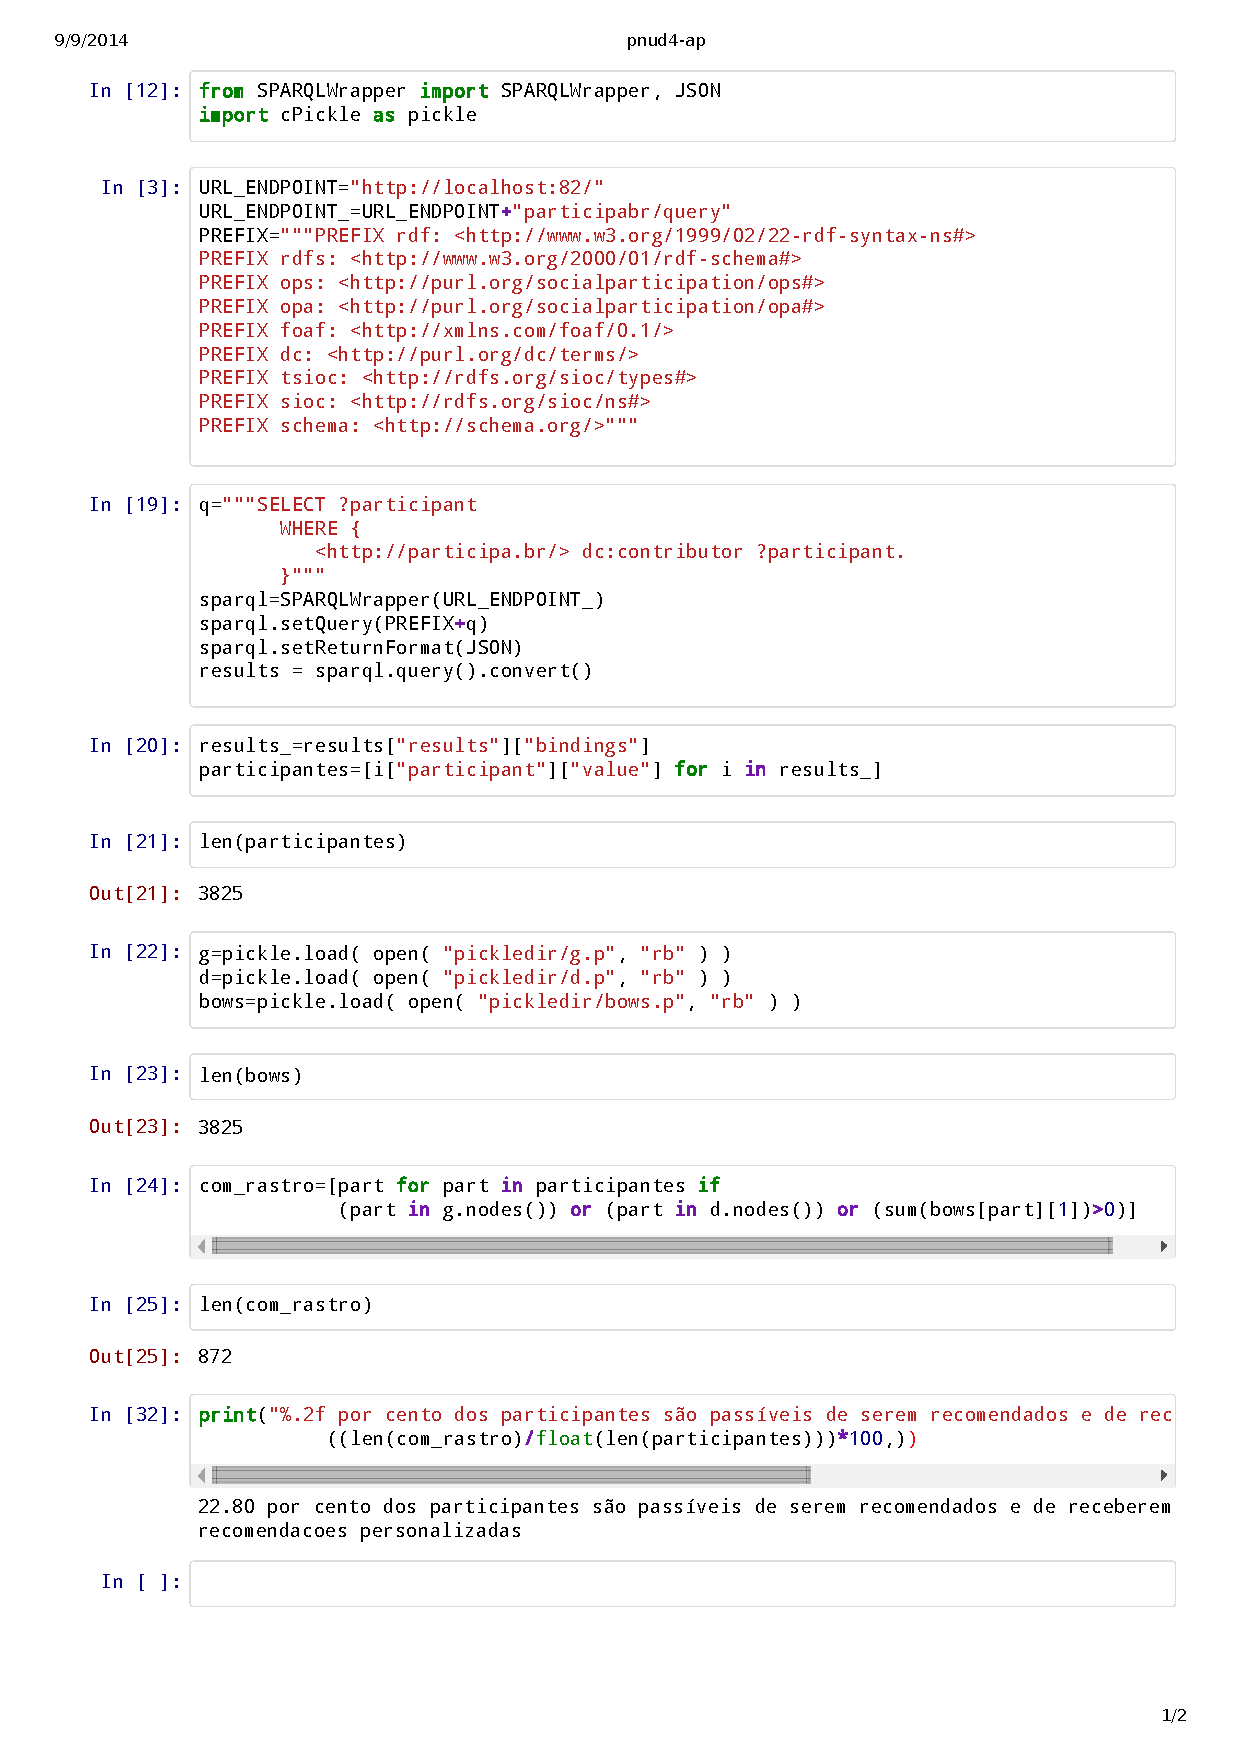
\includepdf[pages=-]{anexos/pnud4-ap.pdf}
\section{Infraestrutura do sistema de recomendações}\label{sec:infra}
A estrutura geral em software e hardware está delineada na subseção~\ref{subsec:hs}
e é tema de todo este documento. Este apêndice descreve os scripts
do sistema de recomendação.

O sistema usufrui do endpoint SparQL para adquirir os dados. O usuário/cliente
do sistema de recomendação acessa URLs via HTTP e recebe JSON, da forma usual.
As rotinas de recomendação em si estão no Apêndice~\ref{sec:algs}. Dada a maturidade
das bibliotecas em Python, a facilidade de desenvolvimento e a capacidade
da comunidade em aproveitar scripts simples na linguagem, todo o sistema de recomendação
está em Python. O servidor HTTP feito em Flask, o acesso ao endpoint SparQL (jena) pelo
SPARQLWrapper, o processamento de linguagem natural em NLTK, os aproveitamentos
das redes complexas em NetworkX. Bibliotecas padrão da linguagem (\emph{builtin} na \emph{Python Standard Library}),
e que estão em uso no sistema de recomendação,
são: json, cPickle, string, random, \_\_builtin\_\_.

O sistema está na pasta flask/ do repositório público~\cite{repoProd4}.
As bibliotecas podem todas serem instaladas via pip e, para iniciar o sistema,
basta chamar \texttt{\$ python recomenda.py} ou apontar o apache para a pasta via WSGI.
O sistema aproveita os binários inclusos ou levará até 30 minutos para iniciar com dados mais recentes, pois é necessária a criação das estruturas auxiliares
descritas na seção~\ref{subsec:com}. Este tempo de processamento é um dos principais motivadores para incluir estas estruturas nos dados triplificados, disponíveis no endpoint SparQL.

Pode-se considerar os arquivos do sistema de recomendação, disponíveis na pasta flask/, assim:
\begin{itemize}
    \item \texttt{configuracao.py}: variáveis de configuração utilizadas em mais de um arquivo, como a URL do endpoint SparQL, as stopwords consideradas, os caracteres desconsiderados e os prefixos (namespaces) usados para as consultas SparQL. Atualmente \href{https://github.com/ttm/pnud4/blob/master/flask/configuracao.py}{o script} possui menos de 20 linhas de código.
    \item \texttt{auxiliar.py}: rotinas de criação das estruturas auxiliares. Por hora são quatro: 1) redes de amizade e 2) de interação. 3) Histograma de palavras usadas em todo participa.br e 4) por cada usuário. Atualmente \href{https://github.com/ttm/pnud4/blob/master/flask/auxiliar.py}{o script} possui $\approx 150$ linhas de código.
    \item \texttt{rotinasRecomendacao.py}: as rotinas de recomendação de recursos propriamente ditas. Utilizam as estruturas auxiliares e opções dadas pelo usuário/cliente. Retorna recomendações. Atualmente, \href{https://github.com/ttm/pnud4/blob/master/flask/rotinasRecomendacao.py}{o script} possui mais de 350 linhas de código.
    \item \texttt{recomenda.py}: este arquivo levanta o servidor Flask e repassa as opções escritas na URL (método GET) para as rotinas em \texttt{rotinasRecomendacao.py}. Atualmente, \href{https://github.com/ttm/pnud4/blob/master/flask/recomenda.py}{o script} possui menos de 100 linhas de código.
\end{itemize}

\section{Instalação e modificação do sistema de recomendações}\label{sec:inst}
O sistema de recomendação pode ser instalado em poucos passos. Por exemplo, em um sistema Ubuntu, os seguintes passos são suficientes:
\begin{enumerate}
    \item Clone do repositório: \texttt{\$ git clone http://github.com/ttm/pnud4}.
    \item Na pasta flask/, inicia serviço com \texttt{\$ python recomenda.py} (ou aponta apache para a pasta com wsgi).
    \item Caso necessário, arrumar configurações de acesso ao endpoint SparQL no arquivo \texttt{configuração.py}.
\end{enumerate}

Para fins de uso do sistema de recomendações dentro do Participa.br, é apropriado o uso de infraestrutura dedicada e que assegure a disponibilidade do serviço. Idealmente, este sistema deve estar junto and endpoint SparQL com os dados do participa.br. Para usos em frontends próprios, este mesmo sistema pode ser instalado em servidos de computação em nuvem gratuítos, como o heroku. Este uso de tecnologias leves e bastante difundidas visa facilitar a geração de materiais derivados. O IPython Notebook também se presta a este fim, com as rotinas expostas para execução e modificação pelo visitante que as acessam por browsers usuais (firefox, chromeum)~\cite{iNotebook}.

\section{Propostas de implementações na interface do portal federal de participação social}\label{sec:acr}
Há implementações previstas e implementações propostas para funcionamento interno ao portal federal de participação social (participa.br). Há também implementações em andamento e confluentes com o participa.br, mas para funcionamento externo à instância Noosfero/Participa.br, com autonomia das bases de dados e frontends. Parte destas implementações estão sendo estudadas para o próximo produto desta consultoria.

\subsection{Implementação prevista no participa.br}
O ActionItem~\cite{actionItem}, prevê uma página em que são recomendados
participantes e comunidades para o usuário logado. Os métodos de recomendação apresentados neste Produto são mais formais e aprofundados (e numerosos) do que os requisitados pelo ActionItem. Por outro lado, não estão triplificadas as relações de pertencimento a comunidade, assim como não estão as tags associadas aos usuários e comunidades. Assim, fica prevista a implementação do plugin do participa.pr que disponibiliza uma página com usuários recomendados. Pode haver adaptação do plugin para melhor atender à profundidade e abrangência do sistema de recomendação feito, como para compatibilizar com limitações como a atual ausência de recomendação de comunidades.

Há também a previsão de ampliar o conjunto dos dados triplificados, incluindo tags e o pertencimento às comunidades e permitindo ao atual sistema recomendar comundidades e considerar as tags.

\subsection{Implementações propostas para o participa.br}\label{sec:props}

Como recomendação geral, o consultor propõe que o participa.br tenha seus processos participativos catalizados com recomendações. Os instrumentos para
esta catálise devem ser apresentados ao participante para que ele aproveite o legado para propósitos próprios, como o encontro de parceiros ou grupo que se opõe, ou participantes com propostas e bagagens diferentes.

No sistema de recomendação entregue junto a este Produto, os critérios das recomendações são sempre enviados junto às recomendações em si, na ordem e com pontuação. É solicitado ao exibir o critério de recomendação e opção para mais recomendações sob aquele e outros critérios. O IPython Notebook foi levantado para convidar visitantes à proposição de novas formas de recomendação.

Estes métodos de recomendação são \emph{em geral} ranqueamentos. Estes ranqueamentos podem orientar análises e escolha de participantes para papéis especiais. Em reuniões da equipe do participa.br foram por vezes sugeridas que trilhas participativas tenham etapas com base nestas atribuições fruto de tecnologias e métodos livres, abertos e formais. Por exemplo: conforme~\cite{fabbri2}, os periféricos produzem mais substantivos e podem ficar responsáveis por uma primera etapa de levantamento de tópicos de interesse, como substantivos e termos. Em um segundo momento, os hubs, que produzem mais adjetivos (também segundo~\cite{fabbri2}), podem qualificar estes assuntos de interesse. A construção de textos a partir destes assuntos e qualificações podem ser feitas pelos intermediários, por suas características também diferenciadas, por exemplo por não serem externos na rede como os periféricos mas e tampouco viscerais como os hubs. Estes textos, talvez selecionados, podem ser colocados em consulta pública de comentário por parágrafo, como já utilizado no participa.br.

Para o uso destes critérios para etapas e trilhas participativas, o grupo precisa já possuir atividade/rastro no participa.br (ou instâncias com dados também triplificados), de preferência no próprio grupo. Caso contrário não há como aplicar os critérios pois não há estrutura para ser analisada. Dentre os que já possuem rastro digital (preferencialmente no participa.br, mas podem ser também páginas do facebook ou registros de tweets), o consultor recomenda que estas trilhas sejam concebidas com a comunidade, junto a algum especialista em redes ou participação social. O consultor responsável por este produto se disponibiliza para auxiliar essa interface com a comunidade na criação da trilha e suas etapas, por entender a pertinência do processo, embora esteja além da consultoria em si.

Para grupos sem rastros digitais prévios, pode-se usar estratégias, como a expectativa de que $\approx 5\%$ vai realmente se engajar, pois é a parcela típica de hubs. De forma semelhante, pode-se observar outros grupos do participa e aproveitar abertamente e em comunidade as propriedades.

O consultor recomenda a criação de dashboards para diferentes recursos do participa.br: usuários, comunidades, trilhas, comentários, palavras, etc. Estes dashboards podem ser externos ao participa.br, disponibilizados juntos do sistema de recomendação (em flask) ou em meteor. Caso seja pertinente, estas dashboards podem ter ID liberada pelo sistema do Noosfero para iframes, de forma que interfaces para estatísticas dos recursos estejam prontamente acessíveis, por exemplo, via lightboxes (balões) nas páginas do participa.br.

O consultor considera importante que seja dada alguma visibilidade aos dados que estão sendo doados e aos usos que estão sendo feito, isso para o visitante e para o participante. Talvez através destes dashboards, dos diferentes recursos do Participa.br, seja alcançado um aproveitamento mais generalizado destes bens que são os dados e tecnologias participativos.

Ao visitar a instancia online do participa.br para conceber possibilidades de implementação/aproveitamento de outras recomendações e análises, as possibilidades destacadas pelo consultor são:
\begin{itemize}
    \item Ao clicar na barra verde do rodapé, com número de usuários, tags, comentários e acessos, pode ser aberto um dashboard com uma análise geral do participa, como as recomendações da linha editorial deste Produto, ou análises como as contidas no produto anterior desta consultoria~\cite{repoProd3}.
    \item Junto aos três pilares Participe!, Proponha! e Mobilize!, pode estar Analise!
    \item Na comunidade de ajuda, item Participe!, como estímulo, podem estar apontados dashboards do participa.br como um todo ou da própria comunidade.
    \item Na comunidade de ajuda, item Mobilize!, podem ser disponibilizadas receitas para difusão de informação, como o movimento em direção aos centrais, o uso de centralidades excludentes ou de técnicas de controle de Baràbasi. Estas receitas apontam participantes para serem acionados pelo participante interessado na mobilização, com base nas redes do participa.br ou outras redes doadas ou apontadas por participantes.
    \item Todo artigo, comentário, palavra, além de acesso a um dashboard que analisa aquela instância do recurso, deve poder também ser usado para recomendação de recursos do próprio participa.br. Caso seja pertinente , o consultor poderá auxiliar a implementação destas recomendações a partir de recursos, e os dashboards de cada recurso.
    \item Na página inicial, logo abaixo do campo reservado para trilhas, pode haver um campo para recomendação de recursos, com as opções do sistema de recomendação de recursos, com os critérios expostos e recomendação de aproveitamento.
    \item Na página inicial, nos campos de comunidades e de pessoas, acrescentar, ao lightbox de opções, dados sobre a pessoa ou ao menos um link para o dashboard. Enriquecer as lightboxes dos recursos da página com dados dos ranqueamentos e dashboard.
    \item Na página inicial, observar recomendações atuais dos recursos e aproveitar este novo sistema de recomendações para auxiliar linha editorial (que escolhe o conteúdo de capa do participa.br).
    \item Nas páginas com postagem de blog, disponibilizar uma análise das palavras e radicais mais incidentes e quais estão sendo usadas para classificação (que estão dentre as 400 mais frequentes que são escolhidas). Junto a esta análise, recursos recomendados a partir da postagem e os critérios usados.
\end{itemize}

Duas implementações sugeridas, menos focadas no portal e mais na funcionalidade, são:
\begin{itemize}
    \item Habilitar plugin para etiquetação desenvolvido pela Daniela Feitosa para o Noosfero/Participa.br. Este plugin permitirá a etiquetação de recursos por participantes do participa.br. Essa etiquetação é essencial para a classificação automática e enriquecimento das análises já existentes para o participa.br. A etiquetação por vários participantes pode melhorar em muito a qualidade dos dados etiquetados, representando amostras maiores e mais diversas.
    \item Fomentar mecanismo de doação de dados (tweets, redes do facebook, dados inseridos por formulário, outras redes, etc). Junto a este mecanismo de doação, abrir acesso público aos dados doados. Interfaces como scrapperWiki e IPython Notebook podem facilitar derivação das análises destes dados doados. No fim das contas, esta demanda aponta para um sistema de monitoramendo aberto.
\end{itemize}

Os produtos dos outros consultores também apontam direções valiosas para desenvolvimento. Em especial:
    confluir plugin para personalização de bloco de estatísticas (da página inicial) com as análises propostas neste produto e no produto anterior do consultor.

Há três vetores nos desenvolvimentos propostos:
\begin{itemize}
    \item Dashboards para cada recurso, com as análises entregues via JSON para o participa mediante requisições HTTP.
    \item Uso de qualquer dos recursos para recomendação de outros recursos.
    \item Exposição de roteiros de aproveitamento da rede social do participante e do participa.br para processos participativos, geralmente envolvendo difusão e coleta de informação. Por exemplo: um participante pode acionar pessoas periféricas da sua rede para iniciar um processo amplo de difusão de informação.
\end{itemize}


Para documentação automática da atividade no participa.br, fortalecendo a transparência e a apropriação da democracia participativa, é útil a criação de análises periódicas diárias, semanais, mensais, semestrais, etc. Estas análises podem ser incorporadas na biblioteca digital de participação social.

Assim que a biblioteca digital estiver acessível, o sistema de recomendação para recursos deve contemplar recursos da biblioteca digital, tanto para recomendar recursos do participa.br quanto para serem recomendados a partir de recursos do participa.br.

\subsection{Implementações confluentes com o participa.br}
Potencializada pela web de dados (web 3.0, web semântica, dados linkados),
é pertinente o desenvolvimento rápido e distribuído de utilidades e análises. Neste contexto, além do arcabouço já exposto (endpoint SparQL, servidor Flask, Noosfero/participa.br), cabe a concepção de frontends com desenvolvimento facilitado, de baixo custo e potentes para visualização e construção coletiva de estruturas via streaming. No âmbito desta consultoria, foram feitos diversos aplicativos voltados para streaming de estruturas sociais e visualização. As possibilidades convergiram empiricamente para o uso do Meteor como framework para desenvolvimento em Node.js e D3.js para visualização. Para observar outras redes sociais (e.g. Twitter, Facebook), ambos Python e Node.js mostraram soluções operantes, porém em Python está mais sólida a comunicação com as APIs, além da pronta disponibilidade de ferramentas de ponta para as análises de redes e de linguagem. Como o D3.js é leve e baseado no padrão SVG, e o Meteor é reativo às mudanças no banco de dados, a solução é apropriada para usos coletivos e simultâneos, assim como para streaming de estruturas sociais~\cite{teloes,oscs,mm,mmissa,mynsa}.

Outra implementação recomendada pelo consultor é a triplificação dos dados de outras instâncias (como do portal Cidade Democrática ou do sistema Autorregulação Algorítmica). Deve-se pensar cuidadosamente em como integrar este legado na biblioteca de participação social em concepção pelo SNAS/SGPR, tanto na confluência das catalogações e da produção de conteúdo (análises), quanto na consideração da biblioteca digital para as análises e para a recomendação de recursos.

\subsection{Implementações previstas e o próximo produto da consultoria}
Há diversas formas de realizar o quinto produto desta consultoria. Portanto, abaixo estão apontadas possibilidades decantadas, não metas estabelecidas, passíveis de serem realizadas por diversas partes interessadas na democracia participativa:
\begin{itemize}
    \item Ampliar triplificação dos dados do participa.br com ao menos: 1) relações de ser membro de comunidade, 2) tags relacionadas às comunidades e aos usuários, 3) dados suplementares do campo 11 da tabela profiles (composto)~\cite{bd}.
    \item Levantamento de um vocabulário de participação social. Considerados os vocabulário enviados pelo IPEA, o Decreto 8243/14 (PNPS), Ontologias de Participação Social e do Participa.br (OPS e OPA), e o vocabulário incidente no Participa.br. Disponibilização em SKOS e/ou para D-Space. Epad em~\cite{padVoc}.
    \item Integração deste arcabouço semântico com a biblioteca digital de participação social sendo erigida pela SNAS/SGPR.
    \item Ampliar recomendações para os outros recursos. Implementar métodos apontados pela equipe ou literatura ou elaborados para este caso do participa.br.
    \item Aprofundamento do tratamento linguístico, e.g. com lematização e classes morfossintáticas.
    \item Scripts que, para análise dos dados, use dados de instâncias diferentes através do endpoint sparql que serve os dados do participa.br. Scripts que acessem diferentes endpoints para as análises (eg. dbpedia). Instâncias de integração dos dados do participa.br com outras instâncias (e.g. frontends).
    \item Triplificação dos dados do Cidade Democrática para disponibilização junto aos do participa.br via endpoint SparQL.
    \item Triplificação dos dados da Autorregulação Algorítmica para disponibilização junto ao participa.br via endpoint SparQL.
    \item Estabelecimento de equivalências entre usuários e informação de alias.
    \item Encaixe dos perfis do participa.br nos padrões vCard e FOAF.
    \item Organização da OPA e da OPS com relação à triplificação dos dados.
    \item Triplificação dos dados do AllOurIdeas usado pelo Participa.br, o que inclui as consultas públicas.
    \item Estudo do pwiki e aproveitamento para o sistema de recomendação ou dashboards.
    \item Conjunto de perguntas simples respondidas com consultas ao endpoint SparQL.
    \item Uma página estática com instruções sobre como usar essa inteligência tecnológica disponibilizada pelo participa.br.
    \item Implementação total ou parcial das opções para recomendação relacionadas na Tabela~\ref{tab:srCampos2}, seção~\ref{sec:plan}.
    \item Implementação dos sitema de dashboards, recomendações e receitas de uso, descrito na seção~\ref{sec:props}.
\end{itemize}

\section{Elementos de interface e cronograma de alterações}
Para facilitar apreensão do conteúdo aqui exposto, este apêndice aponta elementos de interface de forma mais visual e com linguagem menos técnica. Também é apresentado um cronograma para adaptações e incrementos para a interface do portal.
\subsection{Elementos de interface}
São apresentados, a seguir, imagens de interfaces entregues junto a este produto, ou importantes para as recomendações aqui encontradas. 
\subsubsection{Endpoint SparQL}
Ponto de acesso aos dados semanticamente enriquecidos do Participa.br. Seções deste documento que tratam desta interface são~\ref{sec:sfoo} e o Apêndice~\ref{sec:inb}. A Figura~\ref{fig:sparql} é um screenshot da interface gráfica do endpoint sparql em uso, com a resposta típica como na Figura~\ref{fig:sparqlResp}. O endpoint também é acessado por scripts e interfaces como as apresentadas nas seções~\ref{sec:inb} e ~\ref{sec:api}.

\begin{figure}[h!]
  \centering
      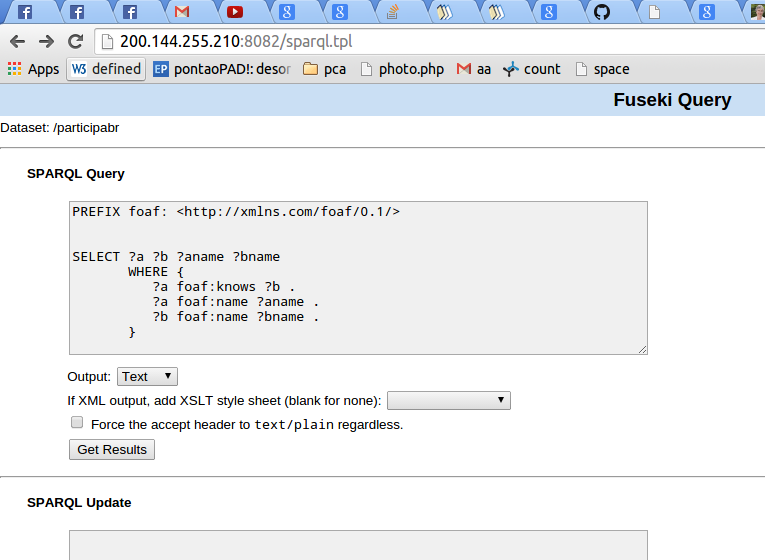
\includegraphics[width=0.8\textwidth]{screenshots/sparql}
  \caption{Interface (Fuseki/Jena) para acesso aos dados enriquecidos semanticamente do participa.br via buscas SparQL. A resposta para esta query é apresentada na Figura~\ref{fig:sparqlResp}}\label{fig:sparql}
\end{figure}


\begin{figure}[h!]
  \centering
      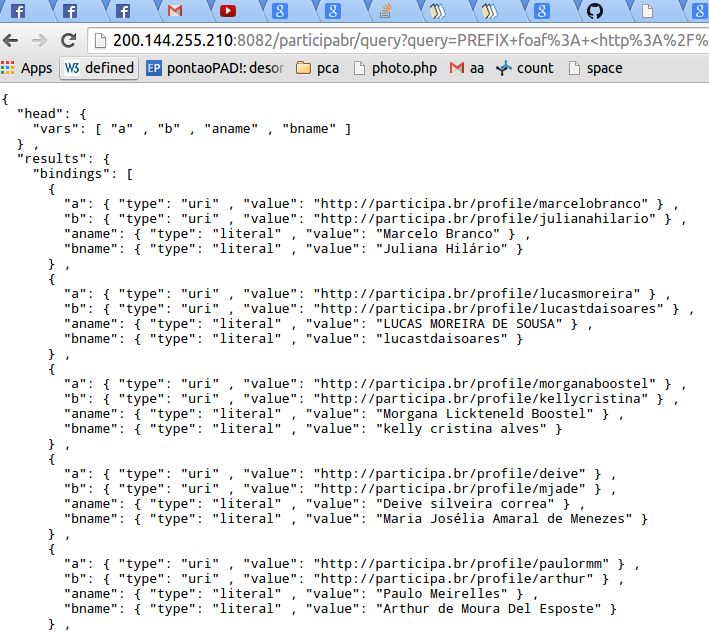
\includegraphics[width=0.8\textwidth]{screenshots/sparqlResp}
  \caption{Resposta em JSON típica em buscas SparQL. Esta imagem reproduz a tela com a resposta à busca da Figura~\ref{fig:sparql}}\label{fig:sparqlResp}
\end{figure}

\subsubsection{IPython Notebook}\label{sec:inb}
Para expor as rotinas de análise e de recomendação dos dados do participa.br, e para facilitar o estudo e a geração de rotinas derivadas, foi disponibilizada uma interface gráfica dedicada: o IPython Notebook. Esta interface possui uma listagem das páginas de anotação disponibilizadas (veja a Figura~\ref{fig:inb1}) e a página de anotação propriamente dita, onde estão as rotinas em Python, resultados e anotações (veja Figura~\ref{fig:inb2}. A seção~\ref{sec:inb5} e o Apêndice~\ref{sec:inb} deste documento tratam desta interface explicitamente.

\begin{figure}[h!]
  \centering
      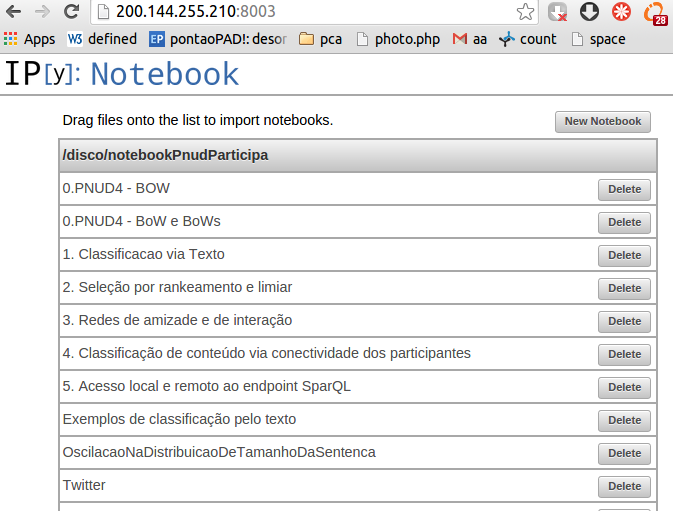
\includegraphics[width=0.8\textwidth]{screenshots/inb1}
  \caption{Página com o índice das anotações da interface para disponibilização online e reativa das rotinas computacionais para tratamento, análise e recomendação de recursos do participa.br. A Figura~\ref{fig:inb2} mostra uma das telas de anotação, em que o visitante pode observar as rotinas, executá-las e até alterá-las para fins de estudo ou proposição de rotinas derivadas.}\label{fig:inb1}
\end{figure}


\begin{figure}[h!]
  \centering
      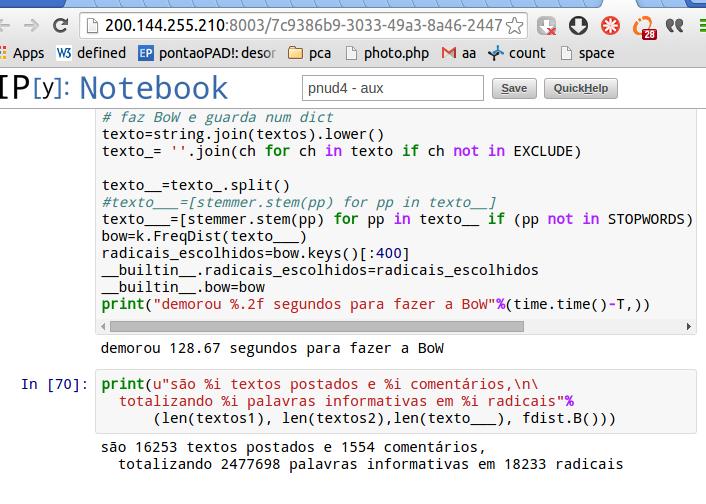
\includegraphics[width=0.8\textwidth]{screenshots/inb2}
  \caption{Página com rotinas reativas e online, uma parte de uma das instâncias listadas no índice da Figura~\ref{fig:inb1}}\label{fig:inb2}
\end{figure}

\subsubsection{API HTTP}\label{sec:api2}
A interface HTTP para recomendações de recursos do participa.br não é uma interface gráfica e ainda não possui um frontend gráfico. Mesmo assim, é uma interface e salienta elementos de usabilidade. A Figura~\ref{fig:api} exibe a interface em funcionamento. A seção~\ref{sec:api3} e o Apêndice~\ref{sec:api} tratam em maiores detalhes esta interface.
\begin{figure}[h!]
  \centering
      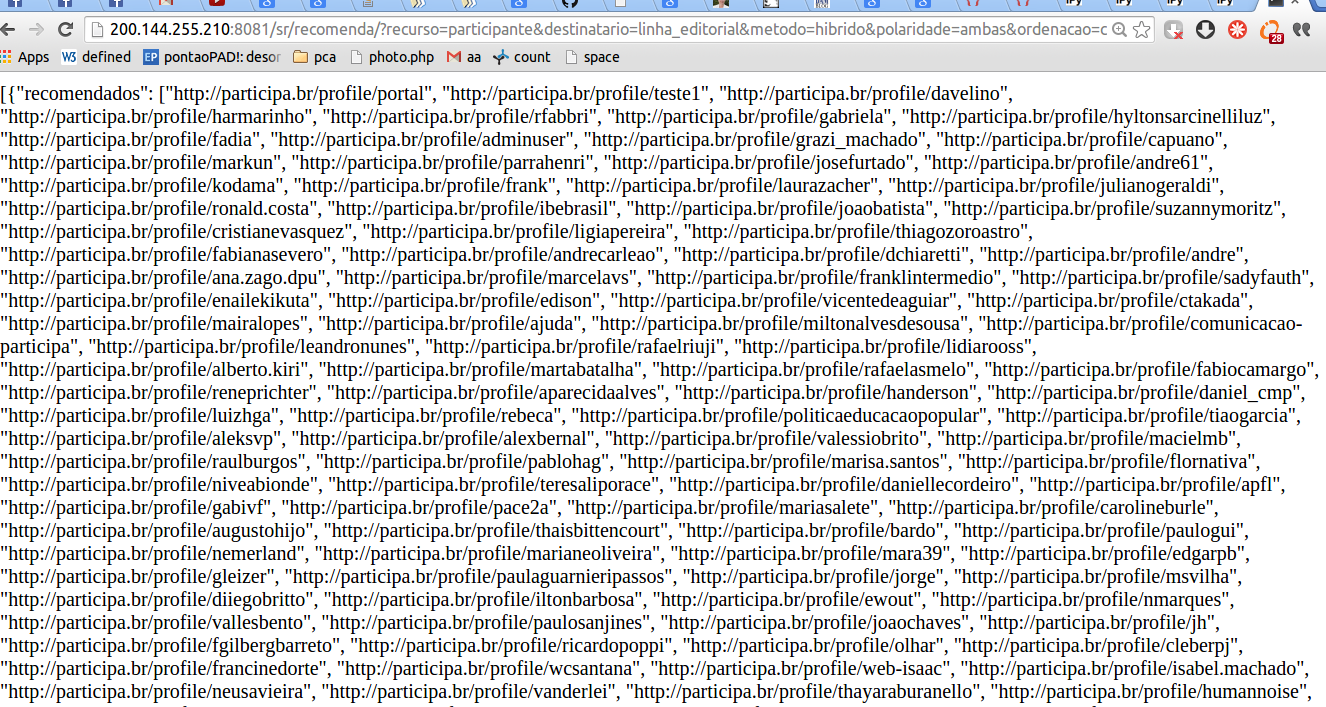
\includegraphics[width=0.8\textwidth]{screenshots/api}
  \caption{Interface HTTP para os sistema de recomendações do participa.br: a consulta é feita pela parametrização da URL acessada (``parâmetros GET''), a resposta é JSON usual.}\label{fig:api}
\end{figure}

\subsubsection{Screenshots de elementos relevantes do Participa.br}
Há diversos elementos visuais do participa.br que são diretamente relacionados às recomendações aqui apresentadas. Isso é esperado, já que está sendo proposto um sistema de recomendação de recursos genérica do participa.br. Bons exemplos de elementos visuais do participa.br estão nas Figuras~\ref{fig:elp1} e~\ref{fig:elp2}, em que maiores detalhes podem ser incluídos na própria interface (ou por redirecionamento) e recursos podem ser recomendados, via métodos diversos, com base no participante escolhido. Estes elementos são considerados com mais especificidade no Apêndice~\ref{sec:acr} e usados no cronograma do Apêndice~\ref{sec:cron}.

\begin{figure}[h!]
  \centering
      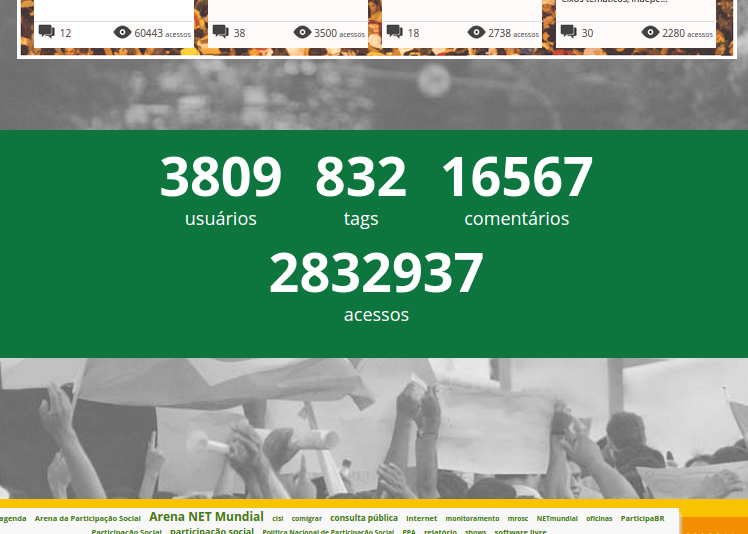
\includegraphics[width=0.8\textwidth]{screenshots/elp1}
  \caption{Barra de estatísicas do participa.br. Esta barra pode exibir mais dados por padrão, via menu dropdown, via informações transitórias que surgem quando o mouse está encima do elemento, ou via link para página externa (para um painel/dashboard do participa.br).}\label{fig:elp1}
\end{figure}

\begin{figure}[h!]
  \centering
      
\includegraphics[width=0.4\textwidth]{screenshots/elp2}
  \caption{Usuário do participa.br e o menu para mais informações ou navegação com base no usuário. Pode-se incluir informações adicionais neste menu, recomendações ou link para interface/página dedicada à análise e navegação pautada pela atuação do usuário escolhido.}\label{fig:elp2}
\end{figure}



\subsection{Cronograma de alterações}\label{sec:cron}
O desenvolvimento do Participa.br conta com equipes de desenvolvimento. Trata-se do desenvolvimento da plataforma Noosfero, com tecnologias específicas, como RoR, e convenções da plataforma, que é um CMS de considerãvel complexidade.

Este produto consiste, segundo o TR, em uma ``proposta de adaptações e incrementos para a interface do portal'', o que consta de forma condensada no Apêndice~\ref{sec:acr} e permeia todo este presente documento. Um passo a passo da implementação no Noosfero em Ruby é objeto de interesse das equipes de desenvolvimento que estão nisso e, segundo entendimento deste consultor e da equipe do Participa.br, foge ao escopo desta consultoria. Por outro lado, uma organização de implementações pode ser delineada pelo consultor, como contribuição inicial para um planejamento de implementação. Esta organização está na Tabela~\ref{crono}.
\begin{table}
\centering
\begin{tabular}{ | c || c | c | c | c | c |}\hline
etapa & set & out & nov & dez & jan-jun \\\hline\hline
1 & $\bullet$ & $\bullet$ & & & \\\hline
2 & $\bullet$ & $\bullet$ & & & \\\hline
3 & & $\bullet$ & & & \\\hline
4 & & & $\bullet$ & & \\\hline
5 & & & $\bullet$ & & \\\hline
6 & & & & $\bullet$ & \\\hline
7 & & & & $\bullet$ & $\bullet$ \\\hline
\end{tabular}
\caption{Contribuição inicial para um cronograma de implementação das recomendações apontadas neste documento. As etapas estão explicitadas na seção~\ref{sec:cron}}
\label{crono}
\end{table}

Etapas:
\begin{enumerate}
    \item Adianto das estruturas auxiliares e algoritmos básicos para a busca dos dados, analise dos recursos e recomendações.
    \item Ativação do plugin para triplificação dos dados na instância do participa.br (plugin já feito, agradecimento à Daniela Feitosa).
    \item Reuniões e amadurecimentos com desenvolvedores ou chefes de equipe para delinear implementações com base na pertinência e possibilidade.
    \item Desenvolvimento de aproveitamentos na interface do Participa.br, como das Figuras~\ref{fig:elp1},~\ref{fig:elp2}. (ao menos das estatísticas ao final e dos dropdown dos participantes).
    \item Término da implementação do plugin de recomendação de perfis do participa.br.
    \item Ativação do plugin na instância atual do Participa.br.
    \item Desenvolvimento do sistema de navegação dos recursos, com dashboards (paineis), métodos de recomendação, registro de potenciais utilidades dos recursos e recomendações, assim como possibilidade de anotação pelos usuários.
\end{enumerate}

As análises (e outras rotinas de processamento de dados) estão em grande parte prontas nos algorítmos apresentados neste produto e no produto anterior. O consultor planeja entregar uma implementação da estrutura de dados completa do sistema de navegação, realizada a partir dos dados enriquecidos semanticamente (etapa 2). Também planeja uma interface (frontend) dedicada, independente do Participa.br, para facilitar testes e usos.

O consultor pode entrar no desenvolvimento do Noosfero/Participa.br, em RoR, e talvez o faça neste produto. Por hora, as equipes de desenvolvimento e a coordenação do participa.br tem afirmado serem mais úteis os esforços do consultor na linha dos dados e análises, por exigirem habilidade e conhecimentos em fronteiras afins com interesses do consultor.

\end{document}
